\documentclass[czech]{beamer}
\usepackage[czech]{babel}
\usepackage[utf8]{inputenc}
\usepackage{hyperref}
\usepackage{algorithmic}
\usepackage[vlined,czech]{algorithm2e}
\SetAlFnt{\small}

\usetheme{Madrid}

\title{Grafové algoritmy - Dijkstrův algoritmus}
\author{Martin Litwora}
\centering
\date{2020}
\begin{document}
\maketitle
\begin{frame}{Obsah}
\begin{itemize}
\item Co je Dijkstrův algoritmus? 
\item Pseudokód
\item Složitost algoritmu 
\item Popis algoritmu
\item Zdroje
\end{itemize}
\end{frame}

\begin{frame}{Dijkstrův algoritmus}
\begin{itemize}
    \item Dijkstrův algoritmus je nejrychlejší známý algoritmus pro nalezení všech nejkratších cest ze zadaného uzlu do ostatních uzlů grafu, \linebreak který neobsahuje hrany záporné délky.
    \item Algoritmus byl vymyšlen nizozemským informatikem Edsgerem Dijkstrou v roce 1959.
    \item Založen na tom, že na začátku přiřadíme uzlům určité hodnoty a postupně jej budeme vylepšovat.
\end{itemize}
\end{frame}

\begin{frame}{Pseudokód}
\begin{algorithm}[H]
\begin{algorithmic}[1]
\FOR{each vertex $V$ in $G$}
\STATE distance$[V] \leftarrow $  infinite
\STATE previou$[V] \leftarrow $ NULL
\IF{$V \neq S$}
\STATE add $V$ to Priority Queue $Q$
\ENDIF
\ENDFOR
\WHILE{$Q$ is not empty}
\STATE $U \leftarrow$ Extract MIN from $Q$
\FOR{each unvisited neighbour $V$ of $U$}
\STATE tmpDistance $\leftarrow$ distance[$U$] + edge\textunderscore weight$(U, V)$
\IF{tmpDistance $\leftarrow$ distance[$V$]}
\STATE distance[$V$] $\leftarrow$ tmpDistance
\STATE previous[$V$] $\leftarrow$ $U$
\ENDIF
\ENDFOR
\ENDWHILE
\RETURN distance[ ], previous[ ]
\end{algorithmic}
%\caption{Pseudokód Dijkstrova algoritmu}
\end{algorithm}
\end{frame}

\begin{frame}{Složitost algoritmu}
\begin{block}{Běžné grafy}
    Nejjednodušší implementace Dijkstrova algoritmu používá pro uložení prioritní fronty pole a operace \emph{Extract MIN($Q$)} je lineární prohledávání všech vrcholů v $Q$. V tomto případě je asymptotická časová složitost $O ( | V | 2 + | E | )$, kde $| V |$ je počet vrcholů a  $| E |$ počet hran. 
\end{block}
\begin{block}{Řídké grafy}
    Pro řídké grafy (grafy s počtem hran mnohem menším než $| V |^2$)  může být Dijkstrův algoritmus implementován mnohem efektivněji tím, že se graf ukládá pomocí seznamu sousedů a funkce \emph{Extract MIN} se implementuje pomocí \emph{binární} nebo \emph{Fibonacciho haldy}. \newline Poté algoritmus běží v čase $O ( ( | E | + | V | ) \log | V | )$, \emph{Fibonacciho halda} se zlepší na $O ( | E | + | V | \log | V | )$.
\end{block}
\end{frame}

\begin{frame}{Popis algoritmu}
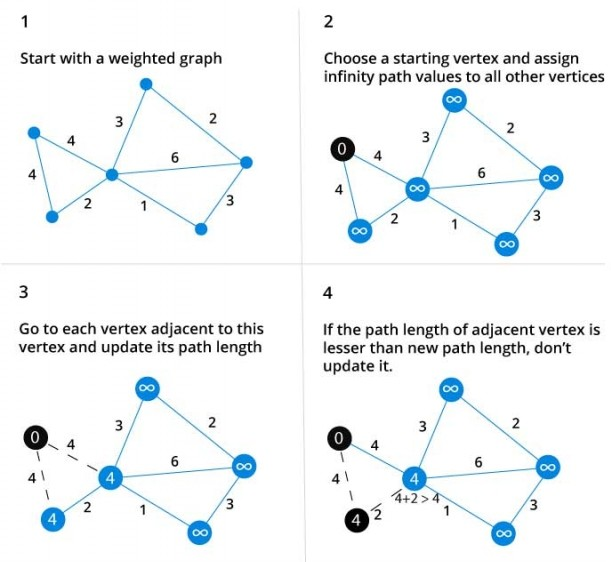
\includegraphics[height=7.5cm]{Dijkstra's-algorithm-1.jpg}
\centering
\end{frame}

\begin{frame}{Popis algoritmu}
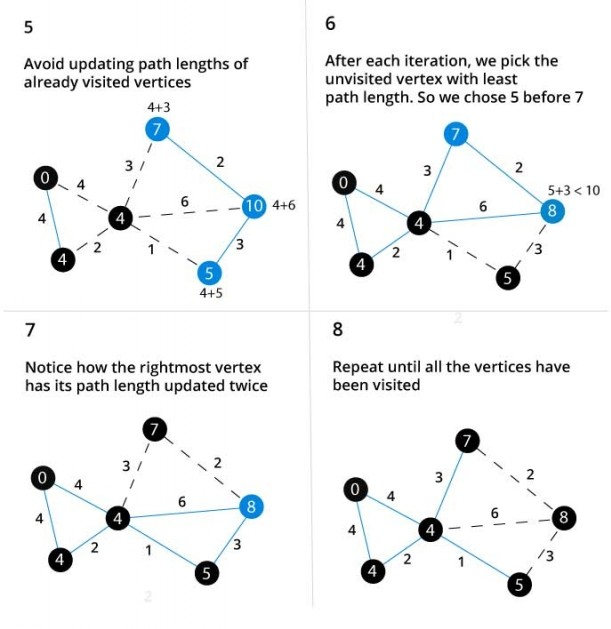
\includegraphics[height=7.5cm]{Dijkstra's-algorithm-2.jpg}
\centering
\end{frame}

\begin{frame}{Zdroje}
    \begin{itemize}
        \item \url{https://cs.wikipedia.org/wiki/Dijkstr\%C5\%AFv_algoritmus}
        \item \url{https://www.programiz.com/dsa/dijkstra-algorithm}
        \item \url{https://cdn.programiz.com/sites/tutorial2program/files/Dijkstra\%27s-algorithm.jpg}
    \end{itemize}
    
\end{frame}

\begin{frame}
    \huge{\centerline{Děkuji za pozornost}}
\end{frame}

\end{document}
